\documentclass[11pt]{report}

\usepackage[left=0.75in, right=0.75in, top=0.75in, bottom=0.75in]{geometry}
\usepackage{layout}
\usepackage{ucs}
\usepackage[utf8x]{inputenc}
\usepackage{titlesec}
\usepackage{graphicx}
\usepackage{amssymb}
\usepackage{amsmath}
\usepackage{dsfont}
\usepackage{float}
\usepackage{caption}
\usepackage{subcaption}
\usepackage{array}



\title{\textbf{TS114 Project}\\Computer-aided analysis of electrocardiogram signals}
\author{{Maxime PETERLIN - Gabriel VERMEULEN }\\\\{ENSEIRB-MATMECA, Bordeaux}}
\date{June, 6th 2014}


\begin{document}


\maketitle

\tableofcontents

\newpage
\vspace{1in}
\vspace{1in}
\section*{\Huge{Introduction}}
	\vspace{0.5in}
	The heart has always been an acurate indicator of one's health. Analyzing it and monitoring its activity is of utmost importance for clinicians. Thus this project's aim is to develop an automatic and user-friendly application capable of giving useful information about the heart activity, such as the cardiac rhythm or the detection of heart conditions, based on an electrocardiogram signal.\\\\
	The project is divided in multiple parts. First, different ECG signals (from both ill and healthy people) were displayed and analysed under MATLAB to highlight their characteristics. Followed by the automated detection of the latter, as well as the identification of cardiac pathologies and the ECG signals denoising. Finally, the ultimate product is delivered with a Graphical User Interface (GUI) making it possible to the clinicians to use it easily and intuitively.\\


\chapter{ECG visualization}
	In this first part, seven different ECG signals will be analyzed and displayed under MATLAB. \\Three of these are records from healthy patient's heart, whereas the other four are from ill ones, each with different pathologies.\\
	This part's aim is to study these signals in the frequency and time domain, starting by the latter, and underline the different caracteristics and properties of these.

	\section{Time display}
		\begin{figure}[ht]
			\centering
			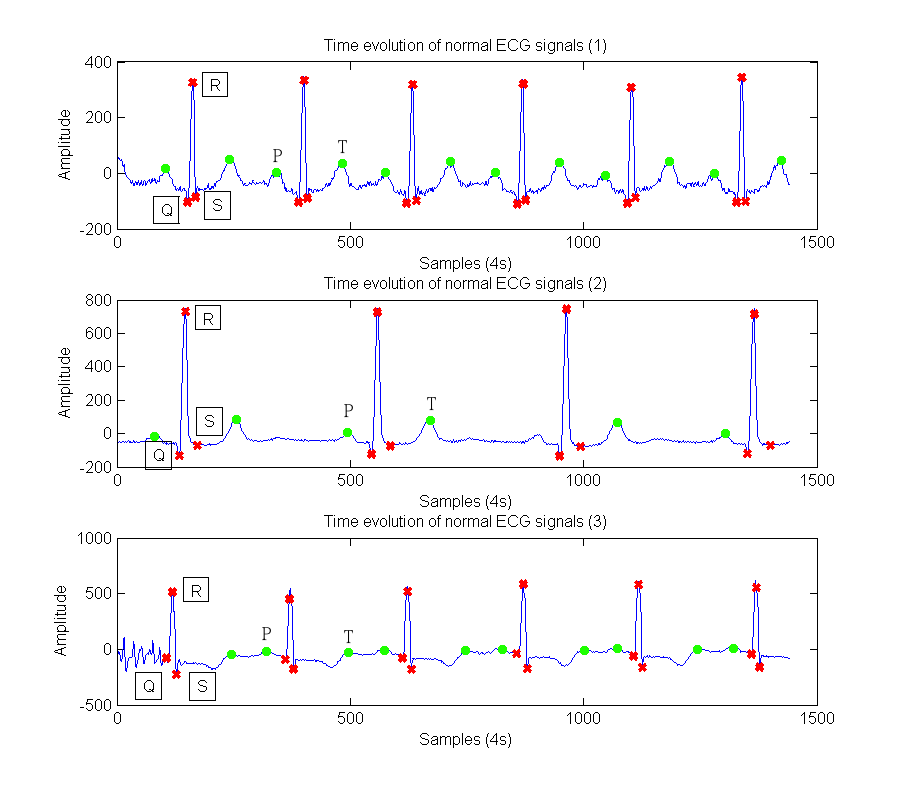
\includegraphics[scale=0.65]{images/Q311_1.png}
			\caption{Normal ECG signals with the Q, R, S points and P, T waves highlighted}
			\label{Q311_1}
		\end{figure}

		First, three seconds of each of the aforementioned normal ECG signals (i.e. from healthy heart) were plotted under MATLAB. On the figure above (Figure~\ref{Q311_1}), their Q, R and S points are represented by red dots, while their P and T waves are located by green dots.  \\
		\\
		The first signal displayed is noisier than the two others, although, its characteristic points and waves are easier to observe.\\
		The second signal is uncluttered, but the S point is hardly recognizable.\\
		Finally, the P and T waves of the third signal, which is a tad noisy, are nearly overlapping.\\
		\\
		Based on these four seconds samples, the cardiac rhythm of each patients was computed and displayed in the table below.\\
		\begin{center}
			\begin{tabular}{|c|c|c|}
				\hline
				\textbf{Signal number} & \textbf{Cardiac rhythm (bpm)} \\
				\hline
				1 & 91.7 \\ 
				\hline
				2 & 53.0 \\
				\hline
				3 & 86.4 \\
				\hline
			\end{tabular}
		\end{center}
		According to the graphs and the computed cardiac rhythms, it can be assumed that the faster the heartbeat is, the noisier the ECG will be. Indeed, the first signal is the fastest heartbeat's ECG while being the noisiest. The same can be said of the third signal.\\
		Moreover, the second signal represents the ECG of a heart with a slow heartbeat and since it is a normal ECG, it might be the heartbeat of an athletic person (otherwise it could be a heart condition like bradycardia).\\
		\\
		\begin{figure}[ht]
			\centering
			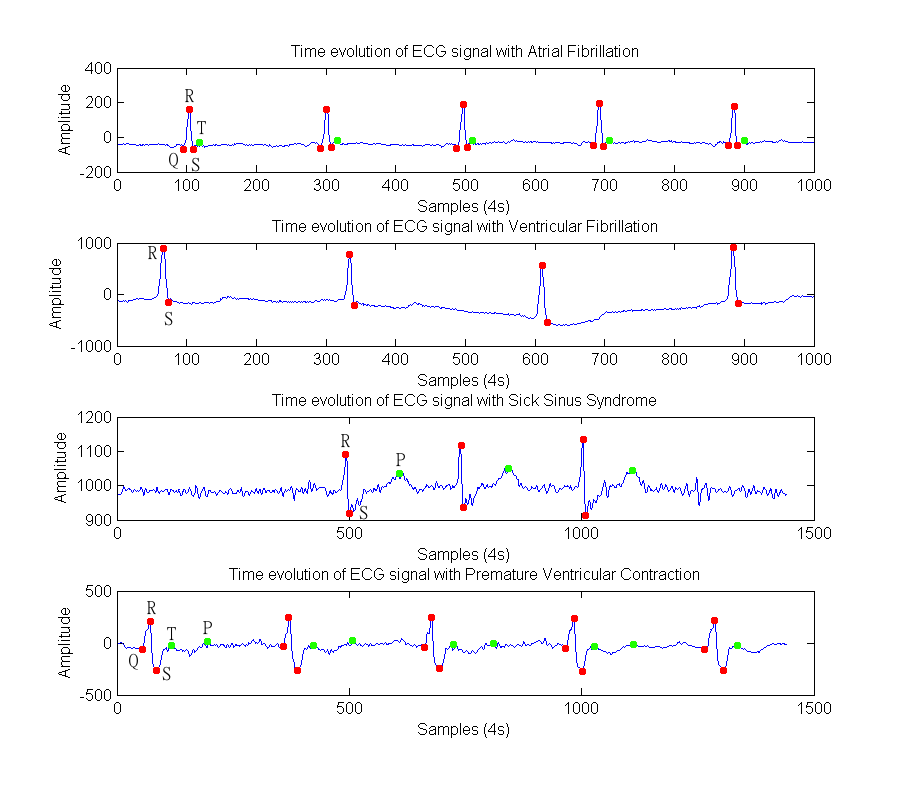
\includegraphics[scale=0.65]{images/Q312_2.png}
			\caption{ECG signals with pathologies with the Q, R, S points and P, T waves highlighted}
			\label{Q312_2}
		\end{figure}
		\\
		Then, the last four ECG signals associated with heart conditions were plotted under MATLAB.\\
		The corresponding cardiac rhythms were computed and displayed in the table below.\\ 
		\begin{center}
			\begin{tabular}{|c|c|c|}
				\hline
				\textbf{Pathology} & \textbf{Cardiac rhythm (bpm)} \\
				\hline
				Atrial Fibrillation & 76.7 \\ 
				\hline
				Ventricular Fibrillation & 55.5 \\
				\hline
				Sick Sinus Syndrome & 84.7 \\
				\hline
				Premature Ventricular Contraction & 71.1 \\
				\hline
			\end{tabular}
		\end{center}
		These pathologies have an impact on each ECG signals and useful characteristics are lost.\\
		Compared to the normal signals, the Atrial Fibrillation's ECG signals lack P waves and has weak impulsions. In the same way, for the Ventricular Fibrillation, the signal depicts a slow heartbeat and hardly discernible P waves, as well as Q and S points.\\
		The Sick Sinus Syndrome has a different effect on the signal, for it creates groups of P waves and R/S points with an absence of activity in between.\\
		The Premature Ventricular Contraction pathology is the closest match, out of the four signals, to a typical one. But, as the pathology's name suggest, the P waves are ahead compared to a normal signal.\\

	\section{Frequency display}
		At first, the ECG power spectrum of the normal ECG signals. $N$ samples were used, with $N = 15 \cdot F_s$.\\
		\\
		\begin{figure}[ht]
			\centering
			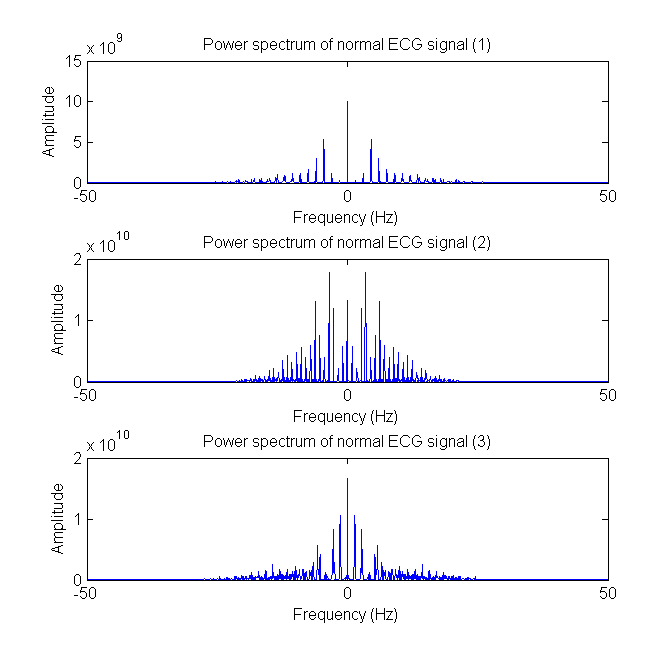
\includegraphics[scale=0.65]{images/Q321.png}
			\caption{ECG power spectrum of the normal ECG signals}
			\label{Q321}
		\end{figure}
		\\
		Since the original signals are periodic, peaks can be found every $f = \frac{n}{T_b}, \forall n \in \mathbb{N}$.\\
		$T_b$ represents the number of beats per second. It is then possible to compute the different cardiac rhythms which are shown in the table below.\\
		\begin{center}
			\begin{tabular}{|c|c|c|}
				\hline
				\textbf{Signal number} & \textbf{Cardiac rhythm (bpm)} \\
				\hline
				1 & 91.8 \\ 
				\hline
				2 & 52.2 \\
				\hline
				3 & 81.9 \\
				\hline
			\end{tabular}
		\end{center}
		The results are pretty close to what was computed in the time domain.\\
		\\
		Then, the signals associated with pathologies were plotted under MATLAB.\\
		\\
		\begin{figure}[ht]
			\centering
			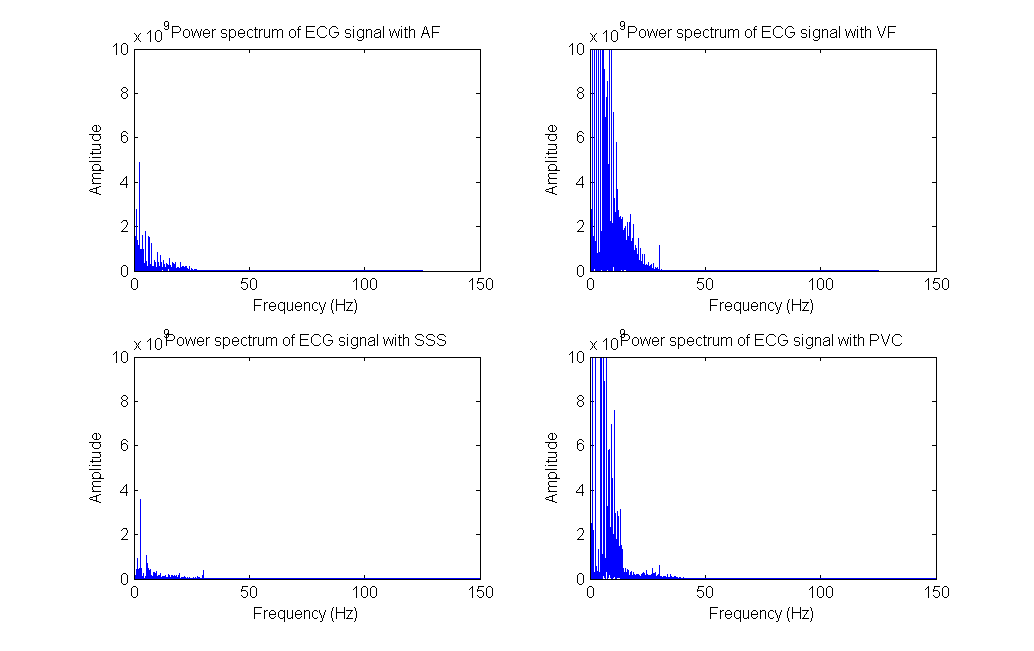
\includegraphics[scale=0.65]{images/Q322.png}
			\caption{ECG power spectrum of the ECG signals associated with pathologies}
			\label{Q322}
		\end{figure}
		\\
		These graphs were cut off, otherwise, since the component in $f = 0$ has a very high value, the scale follow suits and it is almost impossible to see the other components.\\
		The differences between these power spectrum and those from the normal ECG, are firstly, as it was said above, the value of the $f=0$ component.\\
		<< Missing part >>
		\\
		\\
		Out of the previous results, the cardiac rhythm were computed and displayed in the table below. 
		\begin{center}
			\begin{tabular}{|c|c|c|}
				\hline
				\textbf{Pathology} & \textbf{Cardiac rhythm (bpm)} \\
				\hline
				Atrial Fibrillation & 76.8 \\ 
				\hline
				Ventricular Fibrillation & 57.6 \\
				\hline
				Sick Sinus Syndrome & 82.8 \\
				\hline
				Premature Ventricular Contraction & 72 \\
				\hline
			\end{tabular}
		\end{center}
		Just as before, the results match those computed in the time domain.


\chapter{Detection of P, QRS and T waves}
	\section{Three different methods of R waves detection}
		The purpose of this section is to implement and compare three different methods in order to detect the R waves.
		\subsection{Method of local maxima}
			This method is rather straightforward. \\
			First of all, to work on a restricted number of sample, a window is set. The signal is then cubed to make the R waves stand out.\\
			A threshold $r$ is chosen to only select the peaks corresponding to the R waves. $r$ is a variable equal to a certain percentage of the maximum value contained in the ECG signals.\\
			When the peaks are picked, the local maxima of the latter is selected and the corresponding time taken out. Finally, the R points are plotted on the original ECG at the previously found positions.
		\subsection{Method of the derivative}
		\subsection{Pan and Tompkins algorithm}



\chapter{Automatic identification of cardiac pathologies}

\chapter{ECG denoising}


\newpage
\section*{Conclusion}

\end{document}
